\section{Execute Module}

  \begin{figure}[h!]
      \centering
      \vspace{1em}
\scalebox{0.85}{
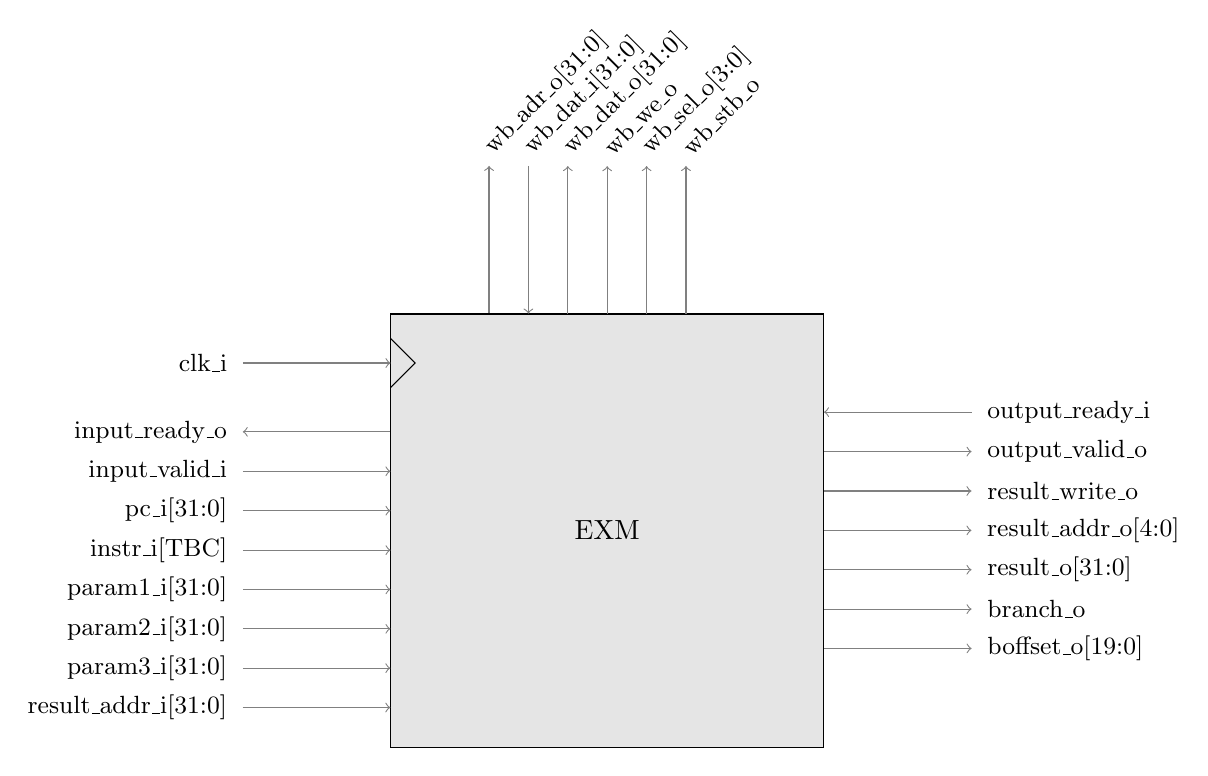
\begin{tikzpicture}[scale=1.25, draw=gray, inner sep=0, outer sep=0]
  \node[rectangle, draw=black,
    anchor=south,
    align=center,
    minimum height = 5.5cm,
    minimum width = 5.5cm,
    fill = gray!20] (block) at (0, 0) {EXM};

  \node (rport4) at (block.east) {};
  \node (rport3) at ([yshift=0.4cm]rport4.center) {};
  \node (rport2) at ([yshift=0.4cm]rport3.center) {};
  \node (rport1) at ([yshift=0.4cm]rport2.center) {};
  \node (rport5) at ([yshift=-0.4cm]rport4.center) {};
  \node (rport6) at ([yshift=-0.4cm]rport5.center) {};
  \node (rport7) at ([yshift=-0.4cm]rport6.center) {};
  \draw[->] ([xshift=1.5cm]rport1.center) node[right=0.2cm, anchor=west]{\small output\_ready\_i} -- (rport1.center);
  \draw[<-] ([xshift=1.5cm]rport2.center) node[right=0.2cm, anchor=west]{\small output\_valid\_o} -- (rport2.center);
  \draw[<-] ([xshift=1.5cm]rport3.center) node[right=0.2cm, anchor=west]{\small result\_write\_o} -- (rport3.center);
  \draw[<-] ([xshift=1.5cm]rport4.center) node[right=0.2cm, anchor=west]{\small result\_addr\_o[4:0]} -- (rport4.center);
  \draw[<-] ([xshift=1.5cm]rport5.center) node[right=0.2cm, anchor=west]{\small result\_o[31:0]} -- (rport5.center);
  \draw[<-] ([xshift=1.5cm]rport6.center) node[right=0.2cm, anchor=west]{\small branch\_o} -- (rport6.center);
  \draw[<-] ([xshift=1.5cm]rport7.center) node[right=0.2cm, anchor=west]{\small boffset\_o[19:0]} -- (rport7.center);

  \node(uport4) at (block.north) {};
  \node(uport3) at ([xshift=-0.4cm]uport4.center) {};
  \node(uport2) at ([xshift=-0.4cm]uport3.center) {};
  \node(uport1) at ([xshift=-0.4cm]uport2.center) {};
  \node(uport5) at ([xshift=0.4cm]uport4.center) {};
  \node(uport6) at ([xshift=0.4cm]uport5.center) {};
  \node(uport7) at ([xshift=0.4cm]uport6.center) {};
  \draw[<-] ([yshift=1.5cm]uport1.center) node[above=0.2cm, anchor=west, rotate=45]{\small wb\_adr\_o[31:0]} -- (uport1.center);
  \draw[->] ([yshift=1.5cm]uport2.center) node[above=0.2cm, anchor=west, rotate=45]{\small wb\_dat\_i[31:0]} -- (uport2.center);
  \draw[<-] ([yshift=1.5cm]uport3.center) node[above=0.2cm, anchor=west, rotate=45]{\small wb\_dat\_o[31:0]} -- (uport3.center);
  \draw[<-] ([yshift=1.5cm]uport4.center) node[above=0.2cm, anchor=west, rotate=45]{\small wb\_we\_o} -- (uport4.center);
  \draw[<-] ([yshift=1.5cm]uport5.center) node[above=0.2cm, anchor=west, rotate=45]{\small wb\_sel\_o[3:0]} -- (uport5.center);
  \draw[<-] ([yshift=1.5cm]uport6.center) node[above=0.2cm, anchor=west, rotate=45]{\small wb\_stb\_o} -- (uport6.center);

  \node (lport4) at ([yshift=-0.2cm]block.west) {};
  \node (lport3) at ([yshift=0.4cm]lport4.center) {};
  \node (lport2) at ([yshift=0.4cm]lport3.center) {};
  \node (lport1) at ([yshift=0.4cm]lport2.center) {};
  \node (lport5) at ([yshift=-0.4cm]lport4.center) {};
  \node (lport6) at ([yshift=-0.4cm]lport5.center) {};
  \node (lport7) at ([yshift=-0.4cm]lport6.center) {};
  \node (lport8) at ([yshift=-0.4cm]lport7.center) {};

  \draw[<-] ([xshift=-1.5cm]lport1.center) node[left=0.2cm, anchor=east]{\small input\_ready\_o} -- (lport1.center);
  \draw[->] ([xshift=-1.5cm]lport2.center) node[left=0.2cm, anchor=east]{\small input\_valid\_i} -- (lport2.center);
  \draw[->] ([xshift=-1.5cm]lport3.center) node[left=0.2cm, anchor=east]{\small pc\_i[31:0]} -- (lport3.center);
  \draw[->] ([xshift=-1.5cm]lport4.center) node[left=0.2cm, anchor=east]{\small instr\_i[TBC]} -- (lport4.center);
  \draw[->] ([xshift=-1.5cm]lport5.center) node[left=0.2cm, anchor=east]{\small param1\_i[31:0]} -- (lport5.center);
  \draw[->] ([xshift=-1.5cm]lport6.center) node[left=0.2cm, anchor=east]{\small param2\_i[31:0]} -- (lport6.center);
  \draw[->] ([xshift=-1.5cm]lport7.center) node[left=0.2cm, anchor=east]{\small param3\_i[31:0]} -- (lport7.center);
  \draw[->] ([xshift=-1.5cm]lport8.center) node[left=0.2cm, anchor=east]{\small result\_addr\_i[31:0]} -- (lport8.center);

  \node (clk) at ([yshift=-0.5cm]block.north west) {};
  \draw[->] ([xshift=-1.5cm]lport3.center |- clk.center) node[left=0.2cm, anchor=east]{\small clk\_i} -- (clk.center);
  % clk triangle
  \draw[-  , draw=black] ([yshift=0.25cm]clk.center) -- ([xshift=0.25cm]clk.center) -- ([yshift=-0.25cm]clk.center);
\end{tikzpicture}
}

      \caption{Schematic view of the Execute Module}
      \label{fig:exm}
    \end{figure}

  \subsection{Interface}

    \begin{content}
        The execute module implements TBC. The signals are described in table \ref{tab:exm-interface}. 
      \end{content}

    {
  \vspace{0.5em}
  \begin{center}
    \refstepcounter{table}
    Table \thetable: Execute Module interface signals\label{tab:exm-interface}
  \end{center}

\footnotesize
\begin{xltabular}{0.9\textwidth}{|l|c|c|X|}
  \hline
  \cellcolor{gray!20}\textbf{NAME} & \cellcolor{gray!20}\textbf{TYPE} & \cellcolor{gray!20}\textbf{WIDTH} & \cellcolor{gray!20}\textbf{DESCRIPTION} \\
  \hline
  clk\_i & I & 1 & Clock input. \\
  \hline
  \multicolumn{4}{|l|}{\textbf{INPUT LOGIC}} \\
  \hline
  input\_ready\_o & O & 1 & Input handshaking signal asserted when ready to receive inputs. \\
  \hline
  input\_valid\_i & I & 1 & Input handshaking signal asserted when the provided inputs are valid. \\
  \hline
  pc\_i & I & 32 & Program counter of the current instruction. \\
  \hline
  instr\_i & I & TBD & Current instruction. \\
  \hline
  param1\_i & I & 32 & First instruction parameter. \\
  \hline
  param2\_i & I & 32 & Second instruction parameter. \\
  \hline
  param3\_i & I & 32 & Third instruction parameter. \\
  \hline
  \multicolumn{4}{|l|}{\textbf{WISHBONE MASTER}} \\
  \hline
  wb\_adr\_o & O & 32 & Wishbone read address.  \\
  \hline
  wb\_dat\_i & I & 32 & Wishbone read data. \\
  \hline
  wb\_dat\_o & O & 32 & Wishbone write data. \\
  \hline
  wb\_we\_o & O & 1 & Wishbone write-enable. \\
  \hline
  wb\_sel\_o & O & 4 & Wishbone byte selector. \\
  \hline
  wb\_stb\_o & O & 1 & Wishbone handshaking signal asserted when emitting a request. \\
  \hline
  wb\_ack\_i & I & 1 & Wishbone handshaking signal asserted when received data is valid. \\
  \hline
  \multicolumn{4}{|l|}{\textbf{OUTPUT LOGIC}} \\
  \hline
  output\_ready\_i & I & 1 & Output handshaking signal asserted when the destination is ready to receive the output. \\
  \hline
  output\_valid\_o & O & 1 & Output handshaking signal asserted when the output is valid. \\
  \hline
  result\_write\_o & O & 1 & Asserted when the instruction shall store its result. \\
  \hline
  result\_addr\_o & O & 5 & Address of the register where the result shall be stored. \\
  \hline
  result\_o & O & 32 & Instruction result. \\
  \hline
  branch\_o & O & 1 & Branch request. \\
  \hline
  boffset\_o & O & 20 & Branch offset from pc\_i \\
  \hline
\end{xltabular}
}


  \subsection{Specification}

    \subsubsection{Upstream requirements}

      The table \ref{tab:exm-upstream-requirements} outlines the upstream requirements applicable to the Execute Module.

      {
  \vspace{0.5em}
  \begin{center}
    \refstepcounter{table}
    Table \thetable: Upstream requirements applicable to the Execute Module\label{tab:exm-upstream-requirements}
  \end{center}
  
\footnotesize
\begin{xltabular}{0.9\textwidth}{|X|c|}
  \hline
  \cellcolor{gray!20}\textbf{ID} \\
  \hline
  \reqref{F\_LUI\_01} \\
  \hline
  \reqref{F\_LUI\_02} \\
  \hline
  \reqref{F\_AUIPC\_01} \\
  \hline
  \reqref{F\_AUIPC\_02} \\
  \hline
  \reqref{F\_JAL\_01} \\
  \hline
  \reqref{F\_JAL\_02} \\
  \hline
  \reqref{F\_JAL\_03} \\
  \hline
  \reqref{F\_JALR\_01} \\
  \hline
  \reqref{F\_JALR\_02} \\
  \hline
  \reqref{F\_JALR\_03} \\
  \hline
  \reqref{F\_BEQ\_01} \\
  \hline
  \reqref{F\_BEQ\_02} \\
  \hline
  \reqref{F\_BNE\_01} \\
  \hline
  \reqref{F\_BNE\_02} \\
  \hline
  \reqref{F\_BLT\_01} \\
  \hline
  \reqref{F\_BLT\_02} \\
  \hline
  \reqref{F\_BGE\_01} \\
  \hline
  \reqref{F\_BGE\_02} \\
  \hline
  \reqref{F\_BLTU\_01} \\
  \hline
  \reqref{F\_BLTU\_02} \\
  \hline
  \reqref{F\_BGEU\_01} \\
  \hline
  \reqref{F\_BGEU\_02} \\
  \hline
  \reqref{F\_LB\_01} \\
  \hline
  \reqref{F\_LB\_02} \\
  \hline
  \reqref{F\_LB\_03} \\
  \hline
  \reqref{F\_LH\_01} \\
  \hline
  \reqref{F\_LH\_02} \\
  \hline
  \reqref{F\_LH\_03} \\
  \hline
  \reqref{F\_LW\_01} \\
  \hline
  \reqref{F\_LW\_02} \\
  \hline
  \reqref{F\_LBU\_01} \\
  \hline
  \reqref{F\_LBU\_02} \\
  \hline
  \reqref{F\_LBU\_03} \\
  \hline
  \reqref{F\_LHU\_01} \\
  \hline
  \reqref{F\_LHU\_02} \\
  \hline
  \reqref{F\_LHU\_03} \\
  \hline
  \reqref{F\_SB\_01} \\
  \hline
  \reqref{F\_SB\_02} \\
  \hline
  \reqref{F\_SH\_01} \\
  \hline
  \reqref{F\_SH\_02} \\
  \hline
  \reqref{F\_SW\_01} \\
  \hline
  \reqref{F\_SW\_02} \\
  \hline
  \reqref{F\_ADDI\_01} \\
  \hline
  \reqref{F\_ADDI\_02} \\
  \hline
  \reqref{F\_ADDI\_03} \\
  \hline
  \reqref{F\_SLTIU\_01} \\
  \hline
  \reqref{F\_SLTIU\_02} \\
  \hline
  \reqref{F\_XORI\_01} \\
  \hline
  \reqref{F\_XORI\_02} \\
  \hline
  \reqref{F\_ORI\_01} \\
  \hline
  \reqref{F\_ORI\_02} \\
  \hline
  \reqref{F\_ANDI\_01} \\
  \hline
  \reqref{F\_ANDI\_02} \\
  \hline
  \reqref{F\_SLLI\_01} \\
  \hline
  \reqref{F\_SLLI\_02} \\
  \hline
  \reqref{F\_SLLI\_03} \\
  \hline
  \reqref{F\_SRLI\_01} \\
  \hline
  \reqref{F\_SRLI\_02} \\
  \hline
  \reqref{F\_SRLI\_03} \\
  \hline
  \reqref{F\_SRAI\_01} \\
  \hline
  \reqref{F\_SRAI\_02} \\
  \hline
  \reqref{F\_SRAI\_03} \\
  \hline
  \reqref{F\_ADD\_01} \\
  \hline
  \reqref{F\_ADD\_02} \\
  \hline
  \reqref{F\_ADD\_03} \\
  \hline
  \reqref{F\_SUB\_01} \\
  \hline
  \reqref{F\_SUB\_02} \\
  \hline
  \reqref{F\_SUB\_03} \\
  \hline
  \reqref{F\_SLL\_01} \\
  \hline
  \reqref{F\_SLL\_02} \\
  \hline
  \reqref{F\_SLL\_03} \\
  \hline
  \reqref{F\_SLT\_01} \\
  \hline
  \reqref{F\_SLT\_02} \\
  \hline
  \reqref{F\_SLTU\_01} \\
  \hline
  \reqref{F\_SLTU\_02} \\
  \hline
  \reqref{F\_XOR\_01} \\
  \hline
  \reqref{F\_XOR\_02} \\
  \hline
  \reqref{F\_SRL\_01} \\
  \hline
  \reqref{F\_SRL\_02} \\
  \hline
  \reqref{F\_SRL\_03} \\
  \hline
  \reqref{F\_SRA\_01} \\
  \hline
  \reqref{F\_SRA\_02} \\
  \hline
  \reqref{F\_SRA\_03} \\
  \hline
  \reqref{F\_OR\_01} \\
  \hline
  \reqref{F\_OR\_02} \\
  \hline
  \reqref{F\_AND\_01} \\
  \hline
  \reqref{F\_AND\_02} \\
  \hline
\end{xltabular}
}


    \subsubsection{Functional requirements}

  \subsection{Behavior}

    \subsubsection{LUI behavior}

      \begin{content}
          The LUI behavior emits a register write request with the first input value. This value is the sign-extended immediate of the instruction, computed in the decode stage.
        \end{content}

      \begin{figure}[H]
          \centering
          \makeatletter\gdef\dividers{}
\begin{tikztimingtable}[%
    scale=0.7,
    timing/dslope=0.1,
    timing/.style={x=6ex,y=3ex},
    x=6ex,
    timing/rowdist=4ex,
    timing/name/.style={font=\footnotesize},
    timing/u/background/.style={fill=gray!20},
    timing/e/background/.style={fill=gray!20},
]
clk\_i & H 2{C C} L \\
& \divider{Stage inputs} \\
input\_ready\_o    & 2E 2H 2E \\
input\_valid\_i    & 2E 2H 2E \\
param1\_i[31:0]    & 2U 2D{} 2U \\
result\_addr\_i[4:0] & 2U 2D{} 2U \\
& \divider{Stage outputs} \\
output\_ready\_i   & 2E 2H 2E \\
output\_valid\_o   & 2.5E 2H 1.5E \\
result\_write\_o      & 2.5E 2H 1.5E\\
result\_addr\_o[4:0] & 2.5U 2D{result\_addr\_i} 1.5U \\
result\_data\_o[31:0] & 2.5U 2D{param1\_i[31:0]} 1.5U \\
\extracode
% grid
\begin{pgfonlayer}{background}
\begin{scope}[semitransparent ,semithick]
\vertlines[darkgray,dotted]{2, 4}
\dividers
\end{scope}
\end{pgfonlayer}
\end{tikztimingtable}
          \caption{Timing diagram of the LUI behavior of the execute module}
          \label{fig:exm-behavior-lui}
        \end{figure}

    \subsubsection{AUIPC behavior}

      \begin{content}
          The AUIPC behavior computes the sum of the first input with the program counter. This first input is the sign-extended immediate of the instruction, computed in the decode stage.
          
          A register write request is emitted to store the value.
        \end{content}

      \begin{figure}[H]
          \centering
          \makeatletter\gdef\dividers{}
\begin{tikztimingtable}[%
    scale=0.7,
    timing/dslope=0.1,
    timing/.style={x=6ex,y=3ex},
    x=6ex,
    timing/rowdist=4ex,
    timing/name/.style={font=\footnotesize},
    timing/u/background/.style={fill=gray!20},
    timing/e/background/.style={fill=gray!20},
]
clk\_i & H 2{C C} L \\
& \divider{Stage inputs} \\
input\_ready\_o    & 2E 2H 2E \\
input\_valid\_i    & 2E 2H 2E \\
pc\_i[31:0]        & 2U 2D{} 2U \\
param1\_i[31:0]    & 2U 2D{} 2U \\
result\_addr\_i[4:0] & 2U 2D{} 2U \\
& \divider{Stage outputs} \\
output\_ready\_i   & 2E 2H 2E \\
output\_valid\_o   & 2.5E 2H 1.5E \\
result\_write\_o      & 2.5E 2H 1.5E\\
result\_addr\_o[4:0] & 2.5U 2D{result\_addr\_i} 1.5U \\
result\_data\_o[31:0] & 2.5U 2D{\textit{val[31:0]}} 1.5U \\
\extracode
% grid
\begin{pgfonlayer}{background}
\begin{scope}[semitransparent ,semithick]
\vertlines[darkgray,dotted]{2, 4}
\dividers
\end{scope}
\end{pgfonlayer}
\end{tikztimingtable}
\begin{center}
    \scriptsize \textit{val[31:0] : pc\_i[31:0] + param1\_i[31:0]}
\end{center}
          \caption{Timing diagram of the AUIPC behavior of the execute module}
          \label{fig:exm-behavior-auipc}
        \end{figure}

    \subsubsection{Unconditional jump behavior}

      \paragraph{JAL}

      \begin{content}
          The JAL behavior emits a branch request to the address offset provided by the first input.
          
          A register write request is emitted to store the address of the following instruction.
        \end{content}

      \begin{figure}[H]
          \centering
          \makeatletter\gdef\dividers{}
\begin{tikztimingtable}[%
    scale=0.7,
    timing/dslope=0.1,
    timing/.style={x=6ex,y=3ex},
    x=6ex,
    timing/rowdist=4ex,
    timing/name/.style={font=\footnotesize},
    timing/u/background/.style={fill=gray!20},
    timing/e/background/.style={fill=gray!20},
]
clk\_i & H 2{C C} L \\
& \divider{Stage inputs} \\
input\_ready\_o    & 2E 2H 2E \\
input\_valid\_o    & 2E 2H 2E \\
pc\_i[31:0]        & 2U 2D{}  2U \\
param1\_i[31:0]    & 2U 2D{}  2U \\
result\_addr\_i[4:0] & 2U 2D{} 2U \\
& \divider{Stage outputs} \\
output\_ready\_i   & 2E 2H 2E \\
output\_valid\_o   & 2.5E 2H 1.5E \\
branch\_o          & 2.5E 2H 1.5E \\
boffset\_o[19:0]   & 2.5U 2D{input1\_i} 1.5U \\
result\_write\_o      & 2.5E 2H 1.5E\\
result\_addr\_o[4:0] & 2.5U 2D{result\_addr\_i} 1.5U \\
result\_data\_o[31:0] & 2.5U 2D{pc\_i + 4} 1.5U \\
\extracode
% grid
\begin{pgfonlayer}{background}
\begin{scope}[semitransparent ,semithick]
\vertlines[darkgray,dotted]{2, 4}
\dividers
\end{scope}
\end{pgfonlayer}
\end{tikztimingtable}
          \caption{Timing diagram of the jump behavior of the execute module for the JAL instruction}
          \label{fig:exm-behavior-jump-jal}
        \end{figure}

      \paragraph{JALR}

      \begin{content}
          The JALR behavior emits a branch request to the address offset provided by the sum of the first and second input.
          
          A register write request is emitted to store the address of the following instruction.
        \end{content}

      \begin{figure}[H]
          \centering
          \makeatletter\gdef\dividers{}
\begin{tikztimingtable}[%
    scale=0.7,
    timing/dslope=0.1,
    timing/.style={x=6ex,y=3ex},
    x=6ex,
    timing/rowdist=4ex,
    timing/name/.style={font=\footnotesize},
    timing/u/background/.style={fill=gray!20},
    timing/e/background/.style={fill=gray!20},
]
clk\_i & H 2{C C} L \\
& \divider{Stage inputs} \\
input\_ready\_o    & 2E 2H 2E \\
input\_valid\_o    & 2E 2H 2E \\
pc\_i[31:0]        & 2U 2D{}  2U \\
param1\_i[31:0]    & 2U 2D{}  2U \\
param2\_i[31:0]    & 2U 2D{}  2U \\
result\_addr\_i[4:0] & 2U 2D{} 2U \\
& \divider{Stage outputs} \\
output\_ready\_i   & 2E 2H 2E \\
output\_valid\_o   & 2.5E 2H 1.5E \\
branch\_o          & 2.5E 2H 1.5E \\
boffset\_o[19:0]   & 2.5U 2D{\textit{offset[19:0]}} 1.5U \\
result\_write\_o      & 2.5E 2H 1.5E\\
result\_addr\_o[4:0] & 2.5U 2D{result\_addr\_i} 1.5U \\
result\_data\_o[31:0] & 2.5U 2D{pc\_i + 4} 1.5U \\
\extracode
% grid
\begin{pgfonlayer}{background}
\begin{scope}[semitransparent ,semithick]
\vertlines[darkgray,dotted]{2, 4}
\dividers
\end{scope}
\end{pgfonlayer}
\end{tikztimingtable}
\begin{center}
    \scriptsize \textit{offset[19:0] : (param1\_i[31:0] + param2\_i[31:0])[19:0]}
\end{center}
          \caption{Timing diagram of the jump behavior of the execute module for the JALR instruction}
          \label{fig:exm-behavior-jump-jalr}
        \end{figure}

    \subsubsection{Branch behavior}

      \begin{content}
          The branch behavior compares the first two inputs depending on the instruction variant. The BEQ and BNE variants check whether the two inputs are equal or not equal respectively. The BLT and BLTU variants check whether the first input is lower than the second input using a signed and unsigned comparison respectively. The BGE and BGEU variants check whether the first input is greater or equal to the second input using a signed and unsigned comparison respectively.
          
          A branch request is emitted in case of successful comparison, providing the address offset given in the third input.
        \end{content}

      \begin{figure}[H]
          \centering
          {
  \vspace{0.5em}
  \begin{center}
    \refstepcounter{table}
    Table \thetable: Description of the parameters of figure \ref{fig:exm-behavior-branch}.\label{tab:exm-behavior-output-branch}
  \end{center}

\footnotesize
\begin{xltabular}{\textwidth}{|l|l|X|}
  \hline
  \cellcolor{gray!20}\textbf{VARIANTS} & \cellcolor{gray!20}\textbf{PARAMETERS} & \cellcolor{gray!20}\textbf{DESCRIPTION} \\
  \hline
  \multirow{1}{*}{BEQ} & cond = if(param1\_i = param2\_i) 1 else 0 & 1 when the first param is equal to the second param. 0 otherwise. \\ 
  \hline
  \multirow{1}{*}{BNE} & cond = if(param1\_i = param2\_i) 0 else 1 & 1 when the first param is not equal to the second param. 0 otherwise. \\ 
  \hline
  \multirow{1}{*}{BLT} & cond = if(param1\_i $<$ param2\_i) 1 else 0 & 1 when the first param is lower than the second param using a signed comparison. 0 otherwise. \\ 
  \hline
  \multirow{1}{*}{BLTU} & cond = if(unsigned(param1\_i) $<$ unsigned(param2\_i)) 1 else 0 & 1 when the first param is lower than the second param using an unsigned comparison. 0 otherwise. \\ 
  \hline
  \multirow{1}{*}{BGE} & cond = if(param1\_i $\ge$ param2\_i) 1 else 0 & 1 when the first param is greater or equal to the second param using a signed comparison. 0 otherwise. \\ 
  \hline
  \multirow{1}{*}{BGEU} & cond = if(unsigned(param1\_i) $\ge$ unsigned(param2\_i)) 1 else 0 & 1 when the first param is greater or equal to the second param using an unsigned comparison. 0 otherwise. \\ 
  \hline
\end{xltabular}
}

          \caption{Timing diagram of the branch behavior of the execute module}
          \label{fig:exm-behavior-branch}
        \end{figure}

      {
  \vspace{0.5em}
  \begin{center}
    \refstepcounter{table}
    Table \thetable: Description of the parameters of figure \ref{fig:exm-behavior-branch}.\label{tab:exm-behavior-output-branch}
  \end{center}

\footnotesize
\begin{xltabular}{\textwidth}{|l|l|X|}
  \hline
  \cellcolor{gray!20}\textbf{VARIANTS} & \cellcolor{gray!20}\textbf{PARAMETERS} & \cellcolor{gray!20}\textbf{DESCRIPTION} \\
  \hline
  \multirow{1}{*}{BEQ} & cond = if(param1\_i = param2\_i) 1 else 0 & 1 when the first param is equal to the second param. 0 otherwise. \\ 
  \hline
  \multirow{1}{*}{BNE} & cond = if(param1\_i = param2\_i) 0 else 1 & 1 when the first param is not equal to the second param. 0 otherwise. \\ 
  \hline
  \multirow{1}{*}{BLT} & cond = if(param1\_i $<$ param2\_i) 1 else 0 & 1 when the first param is lower than the second param using a signed comparison. 0 otherwise. \\ 
  \hline
  \multirow{1}{*}{BLTU} & cond = if(unsigned(param1\_i) $<$ unsigned(param2\_i)) 1 else 0 & 1 when the first param is lower than the second param using an unsigned comparison. 0 otherwise. \\ 
  \hline
  \multirow{1}{*}{BGE} & cond = if(param1\_i $\ge$ param2\_i) 1 else 0 & 1 when the first param is greater or equal to the second param using a signed comparison. 0 otherwise. \\ 
  \hline
  \multirow{1}{*}{BGEU} & cond = if(unsigned(param1\_i) $\ge$ unsigned(param2\_i)) 1 else 0 & 1 when the first param is greater or equal to the second param using an unsigned comparison. 0 otherwise. \\ 
  \hline
\end{xltabular}
}


    \subsubsection{Load behavior}

      \begin{content}
          The load behavior fetches an 8/16/32-bit word from memory at the address given in the first instruction input for the LB/LBU, LH/LHU and LW instructions respectively. The value is zero-extended to 32-bits for the U variants while it is signed extended to 32-bits otherwise. 
          
          A register write request is then emitted to store the value. 
          
          This behavior induces a pipeline stall due to the memory access time.
        \end{content}

      \begin{figure}[H]
          \centering
          {
  \vspace{0.5em}
  \begin{center}
    \refstepcounter{table}
    Table \thetable: Description of the parameters of figure \ref{fig:exm-behavior-load}.\label{tab:exm-behavior-output-load}
  \end{center}

\footnotesize
\begin{xltabular}{\textwidth}{|l|l|X|}
  \hline
  \cellcolor{gray!20}\textbf{VARIANTS} & \cellcolor{gray!20}\textbf{PARAMETERS} & \cellcolor{gray!20}\textbf{DESCRIPTION} \\
  \hline
  \multirow{2}{*}{LB} & val[31:0] = \{24\{wb\_data\_i[7]\}, wb\_data\_i[7:0]\} & The sign-extended 8-bit data retrieved from memory. \\ \cline{2-3}
  & sel[3:0] = 0b0001 & Only the lowest significant byte is selected. \\
  \hline
  \multirow{2}{*}{LH} & val[31:0] = \{16\{wb\_data\_i[15]\}, wb\_data\_i[15:0]\} & The sign-extended 16-bit data retrieved from memory.  \\\cline{2-3}
  & sel[3:0] = 0b0011 & Only the two lowest significant bytes are selected. \\
  \hline
  \multirow{2}{*}{LW} & val[31:0] = wb\_data\_i[31:0] & The 32-bit data retrieved from memory. \\\cline{2-3}
  & sel[3:0] = 0b1111 & All bytes are selected. \\
  \hline
  \multirow{2}{*}{LBU} & val[31:0] = \{0x000000, wb\_data\_i[7:0]\} & The zero-extended 8-bit data retrieved from memory. \\\cline{2-3}
  & sel[3:0] = 0b0001 & Only the lowest significant byte is selected. \\
  \hline
  \multirow{2}{*}{LHU} & val[31:0] = \{0x0000, wb\_data\_i[15:0]\} & The zero-extended 16-bit data retrieved from memory. \\\cline{2-3}
  & sel[3:0] = 0b0011 & Only the two lowest significant bytes are selected. \\
  \hline
\end{xltabular}
}

          \caption{Timing diagram of the load behavior of the execute module}
          \label{fig:exm-behavior-load}
        \end{figure}

      {
  \vspace{0.5em}
  \begin{center}
    \refstepcounter{table}
    Table \thetable: Description of the parameters of figure \ref{fig:exm-behavior-load}.\label{tab:exm-behavior-output-load}
  \end{center}

\footnotesize
\begin{xltabular}{\textwidth}{|l|l|X|}
  \hline
  \cellcolor{gray!20}\textbf{VARIANTS} & \cellcolor{gray!20}\textbf{PARAMETERS} & \cellcolor{gray!20}\textbf{DESCRIPTION} \\
  \hline
  \multirow{2}{*}{LB} & val[31:0] = \{24\{wb\_data\_i[7]\}, wb\_data\_i[7:0]\} & The sign-extended 8-bit data retrieved from memory. \\ \cline{2-3}
  & sel[3:0] = 0b0001 & Only the lowest significant byte is selected. \\
  \hline
  \multirow{2}{*}{LH} & val[31:0] = \{16\{wb\_data\_i[15]\}, wb\_data\_i[15:0]\} & The sign-extended 16-bit data retrieved from memory.  \\\cline{2-3}
  & sel[3:0] = 0b0011 & Only the two lowest significant bytes are selected. \\
  \hline
  \multirow{2}{*}{LW} & val[31:0] = wb\_data\_i[31:0] & The 32-bit data retrieved from memory. \\\cline{2-3}
  & sel[3:0] = 0b1111 & All bytes are selected. \\
  \hline
  \multirow{2}{*}{LBU} & val[31:0] = \{0x000000, wb\_data\_i[7:0]\} & The zero-extended 8-bit data retrieved from memory. \\\cline{2-3}
  & sel[3:0] = 0b0001 & Only the lowest significant byte is selected. \\
  \hline
  \multirow{2}{*}{LHU} & val[31:0] = \{0x0000, wb\_data\_i[15:0]\} & The zero-extended 16-bit data retrieved from memory. \\\cline{2-3}
  & sel[3:0] = 0b0011 & Only the two lowest significant bytes are selected. \\
  \hline
\end{xltabular}
}


    \subsubsection{Store behavior}

      \begin{content}
          The store behavior writes a 8/16/32-bit word to memory at the address given in the first instruction input for the SB, SH and SW instructions respectively.

          Although there is no need for the pipeline to wait for the data to be written, this behavior induces a pipeline stall in revision 1.0.0 as a write request takes at least two cycles to complete while the memory interface shall be ready to receive new requests in the next pipeline cycle.
        \end{content}

      \begin{figure}[H]
          \centering
          \makeatletter\gdef\dividers{}
\begin{tikztimingtable}[%
    scale=0.7,
    timing/dslope=0.1,
    timing/.style={x=6ex,y=3ex},
    x=6ex,
    timing/rowdist=4ex,
    timing/name/.style={font=\footnotesize},
    timing/u/background/.style={fill=gray!20},
    timing/e/background/.style={fill=gray!20},
]
clk\_i & H 3{C C} L \\
& \divider{Stage inputs} \\
input\_ready\_o            & 2E 2L 2H 2E \\
input\_valid\_i            & 2E 2H 2H 2E \\
param1\_i                  & 2U 4D{}  2U \\
& \divider{Memory access} \\
wb\_clk\_i       & H 3{C C} L \\
wb\_adr\_o[31:0] & 2.5U 4D{param1\_i}  1.5U \\
wb\_dat\_o[31:0] & 2.5U 2U 2D{param2\_i}               1.5U \\
wb\_we\_o        & 2.5E 2H 2H                 1.5E \\
wb\_sel\_o[3:0]  & 2.5U 4D{\textit{sel[3:0]}}                 1.5U \\
wb\_stb\_o       & 2.5E 4H                    1.5E \\
wb\_ack\_i       & 2.5E 2L 2H                 1.5E \\
& \divider{Stage outputs} \\
output\_ready\_i   & 2E 4H 2E \\
output\_valid\_o            & 2.5E 2L 2H 1.5E \\
result\_write\_o    & 2.5E 2L 2L  1.5E\\
\extracode
% grid
\begin{pgfonlayer}{background}
\begin{scope}[semitransparent ,semithick]
\vertlines[darkgray,dotted]{2, 4, 6}
\dividers
\end{scope}
\end{pgfonlayer}
\end{tikztimingtable}

          \caption{Timing diagram of the store behavior of the execute module}
          \label{fig:exm-behavior-store}
        \end{figure}

      \makeatletter\gdef\dividers{}
\begin{tikztimingtable}[%
    scale=0.7,
    timing/dslope=0.1,
    timing/.style={x=6ex,y=3ex},
    x=6ex,
    timing/rowdist=4ex,
    timing/name/.style={font=\footnotesize},
    timing/u/background/.style={fill=gray!20},
    timing/e/background/.style={fill=gray!20},
]
clk\_i & H 3{C C} L \\
& \divider{Stage inputs} \\
input\_ready\_o            & 2E 2L 2H 2E \\
input\_valid\_i            & 2E 2H 2H 2E \\
param1\_i                  & 2U 4D{}  2U \\
& \divider{Memory access} \\
wb\_clk\_i       & H 3{C C} L \\
wb\_adr\_o[31:0] & 2.5U 4D{param1\_i}  1.5U \\
wb\_dat\_o[31:0] & 2.5U 2U 2D{param2\_i}               1.5U \\
wb\_we\_o        & 2.5E 2H 2H                 1.5E \\
wb\_sel\_o[3:0]  & 2.5U 4D{\textit{sel[3:0]}}                 1.5U \\
wb\_stb\_o       & 2.5E 4H                    1.5E \\
wb\_ack\_i       & 2.5E 2L 2H                 1.5E \\
& \divider{Stage outputs} \\
output\_ready\_i   & 2E 4H 2E \\
output\_valid\_o            & 2.5E 2L 2H 1.5E \\
result\_write\_o    & 2.5E 2L 2L  1.5E\\
\extracode
% grid
\begin{pgfonlayer}{background}
\begin{scope}[semitransparent ,semithick]
\vertlines[darkgray,dotted]{2, 4, 6}
\dividers
\end{scope}
\end{pgfonlayer}
\end{tikztimingtable}


    \subsubsection{Arithmetic and logic behavior}

      \begin{content}
          The arithmetic and logic behavior applies to OP and OP-IMM opcodes. As DECM handles the processing of instruction inputs, both OP and OP-IMM instructions have the same associated behavior in EXM.

          The arithmetic and logic behavior computes the following integer operations : signed sum, signed substraction, bitwise exclusive-or, bitwise or, bitwise and, signed comparison, unsigned comparison, left logical shift, right logical shift and right arithmetic shift.
          
          A register write request is then emitted to store the value.
        \end{content}

      \begin{figure}[H]
          \centering
          \makeatletter\gdef\dividers{}
\begin{tikztimingtable}[%
    scale=0.7,
    timing/dslope=0.1,
    timing/.style={x=6ex,y=3ex},
    x=6ex,
    timing/rowdist=4ex,
    timing/name/.style={font=\footnotesize},
    timing/u/background/.style={fill=gray!20},
    timing/e/background/.style={fill=gray!20},
]
clk\_i & H 2{C C} L \\
& \divider{Stage inputs} \\
input\_ready\_o            & 2E 2H 2E \\
input\_valid\_i            & 2E 2H 2E \\
param1\_i                  & 2U 2D{}  2U \\
param2\_i                  & 2U 2D{}  2U \\
& \divider{Stage outputs} \\
output\_ready\_i   & 2E 2H 2E \\
output\_valid\_o            & 2.5E 2H 1.5E \\
result\_write\_o    & 2.5E 2H  1.5E\\
result\_addr\_o[4:0] & 2.5U 2D{result\_addr\_i} 1.5U \\
result\_data\_o[31:0] & 2.5U 2D{\textit{val[31:0]}} 1.5U \\
\extracode
% grid
\begin{pgfonlayer}{background}
\begin{scope}[semitransparent ,semithick]
\vertlines[darkgray,dotted]{2, 4}
\dividers
\end{scope}
\end{pgfonlayer}
\end{tikztimingtable}
          \caption{Timing diagram of the arithmetic and logic behavior of the execute module}
          \label{fig:exm-behavior-arithmetic-logic}
        \end{figure}

      \makeatletter\gdef\dividers{}
\begin{tikztimingtable}[%
    scale=0.7,
    timing/dslope=0.1,
    timing/.style={x=6ex,y=3ex},
    x=6ex,
    timing/rowdist=4ex,
    timing/name/.style={font=\footnotesize},
    timing/u/background/.style={fill=gray!20},
    timing/e/background/.style={fill=gray!20},
]
clk\_i & H 2{C C} L \\
& \divider{Stage inputs} \\
input\_ready\_o            & 2E 2H 2E \\
input\_valid\_i            & 2E 2H 2E \\
param1\_i                  & 2U 2D{}  2U \\
param2\_i                  & 2U 2D{}  2U \\
& \divider{Stage outputs} \\
output\_ready\_i   & 2E 2H 2E \\
output\_valid\_o            & 2.5E 2H 1.5E \\
result\_write\_o    & 2.5E 2H  1.5E\\
result\_addr\_o[4:0] & 2.5U 2D{result\_addr\_i} 1.5U \\
result\_data\_o[31:0] & 2.5U 2D{\textit{val[31:0]}} 1.5U \\
\extracode
% grid
\begin{pgfonlayer}{background}
\begin{scope}[semitransparent ,semithick]
\vertlines[darkgray,dotted]{2, 4}
\dividers
\end{scope}
\end{pgfonlayer}
\end{tikztimingtable}

    \subsubsection{Hazard behaviors}

      \begin{content}
          Hazard behaviors are described in section \ref{pipeline-stall}.
        \end{content}

\newpage
